
\paragraph{} This chapter will cover a number of topics essential to understanding the rationale and implementation of the design as discussed in §~\ref{sec:design}. These include; Intel SGX, a brief overview of modern \textit{libOSes}, an introduction to \textit{Information Flow Control} (\textit{IFC}), and a overview of key aspects of the Linux kernel relevant to the architecture of the prototype.

\section{Intel SGX}

\paragraph{} Intel's Software Guard Extensions, SGX, was first announced and detailed in a handful of whitepaper documents published in 2013. [X,Y,Z] It described a novel approach, creating in-CPU containers with their own protected memory pools. These regions, called \textit{enclaves}, cannot be read from or written due to fundamental protection mechanisms provided by the x86 architecture. \textit{Enclaves} provide both integrity and secrecy to the operation running inside of it, even in the prescence of a malicious host.

\paragraph{Motivation} At a high level SGX aims to achieve security for sensitive application by shielding them, and the resources it uses, against tampering and to provide a guarantee to end users about the an enclaves integrity; this is achieved using measurement and attestation. A driving use case is in a cloud computing context, where users are forced to trust a foreign party with both their data and business logic. By distributing encrypted, yet executable, containers targetting a single, unique SGX CPU, users can be assured that their information is safe, regardless of any virutalisation that may be taking place. Only the provisioned CPU is able to decrypt and execute the enclave, strictly in accordance with the restrictions of the SGX platform.

\subsection{Security Characteristics}

\begin{figure}[]
    \centering
    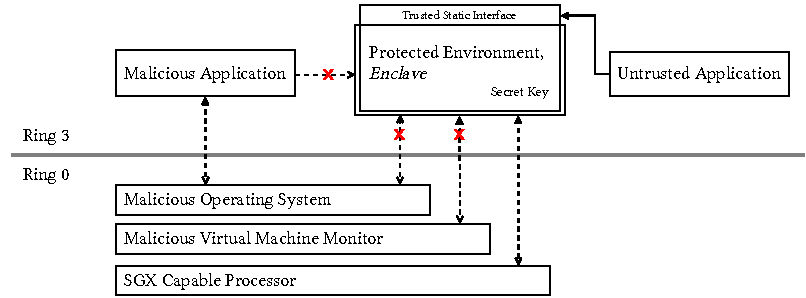
\includegraphics[width=0.9\linewidth]{figures/SGX-architecture.pdf}
    \caption{Abstract overview of an SGX enclave's protections.}
    \label{fig:sgx-basic}
\end{figure}

\paragraph{} At its heart SGX is designed to be \textit{trustworthy}; this is achieved in a number of ways, including robust enclaving provisioning, sealing and attestation. Intel enumerates SGX's protection as follows;

\begin{itemize}
    \item Memory security against observation and modification from outside the enclave; this is achieved using an in-die \textit{Memory Encryption Engine} (\textit{MEE}), with a secret that rotates on every boot. This protection notably works against a host hypervisor, other enclaves, and anything running in supervisor mode.
    \item Attestation of an enclave to a challenger through the use of a permanent hardware security key for asymmetric encryption.
    \item Proxied software calls to prepare and transfer control in and out of an enclave. Arguments are securely marshalled according to a static enclave definition.
    \item SGX does not defend against reverse engineering or sidechannel attacks: [X,Y] this is the responsibility of the developer to mitigate.
    \item Debugging support is only provided via a specialised tool and only when an enclave is compiled with debugging enabled.
\end{itemize}

\subsection{Architecture and Implementation}
\paragraph{} Kernel module, driver. SDK.

\subsection{Enclave Lifecycle}

\subsection{Attestation}

\subsection{Provisioning and Sealing}

\section{Modern \textit{libOSes}}

\section{Information Flow Control}

\section{Aspects of the \textit{Linux} Kernel}